\section{Data used and experimental campaign} \label{campaign}
\subsection{Data}
As said before, this work attempts to find optimal solutions in means of revenue and energy on two kinds of hotel. The first case corresponds to an easily found small scale hotel with one floor and with 20\% of its rooms only dedicated to high level requests. In the scale commented before, six rooms where imposed as low level, 3 as middle range and 1 as high level. The bigger hotel, on the other hand counts with 23 rooms (15 low , 6 medium , 2 high), with 7 of them located on the first floor, and 8 on the other two. This information is necessary for planning the demand.

The optimal analysis should take place every time there is a new request, introducing the already occupied rooms as constraints. For analysis purposes, however, an optimisation horizon of two weeks was proposed. Fig.~\ref{figDemand_stat} shows the distribution used for planning the demand and based on information provided by a marketing analysis from ISTAT \cite{istat} in Liguria. Also, the weather parameters were taken from a Genova weather file, including those of the exterior temperature, ground temperature and solar radiation. \cite{weather}

\begin{figure}[htbp]
	\centering
	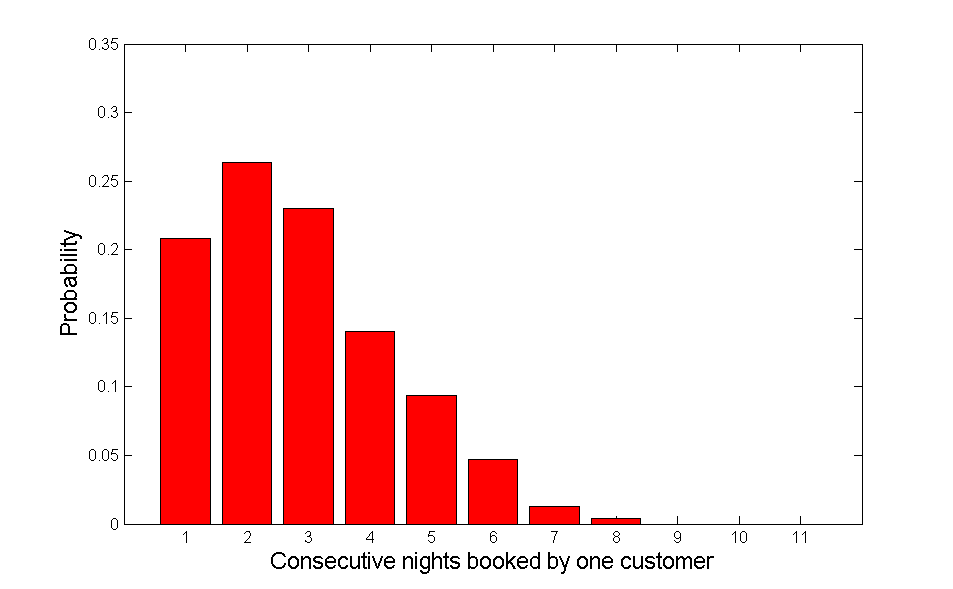
\includegraphics[width=0.45\textwidth, height=0.22\textwidth]{img/Booking_probability1.png}
	\caption{\textit{Statistical distribution of the consecutive number of night asked by a customer.}}
	\label{figDemand_stat}
\end{figure}

As explained before, the revenue is not just dependent on the price of the room, but also on the maintenance costs of the room which is about one tenth of the room's price (1, 3, 8 [$\frac{money}{night}]$). Finally, according to the formulation, a compatible costumer for a room can stay in a upper quality room paying the same price as offered during the booking request. So, since the revenue is the difference between price and maintenance cost of a room, the hotel can get 6 possible revenues according the combinations seen in Table~\ref{tab:profits}.

\subsection{Experimental campaign}
A non-dimensional index was proposed in order to evaluate the performance of the scheduling system against that of common assignment approaches: The Relative Percent Deviation- RPD.
$$RPD = \frac{|X_{o} - X_{r}|}{X_{o}}\times 100$$
Where:
$X_{o}$ is a characteristic measure of the energy obtained by using any assignment ensuring maximum profit.
$X_{r}$ corresponds to the optimal energy solution with maximum revenue as constraint.

An important variable taken into consideration is the percentage occupancy of the hotel. If it were 100\% occupied, there would not be any reason to optimize the assignment of customers. Characteristic rates of approximately 30\%, 50\% and 65\%. Because the demand is generated before optimizing the revenue and some of the requests can be rejected during this step, some extra demand was added in order to remain about the above mentioned values. 

Notice that the optimal energy consumption solution is not compared against any possible assignment given by any solver with non optimizing characteristics but rather against the heuristic solution of the solver used for optimisation (Gurobi). Moreover, to ensure robustness of the analysis form the statistical point of view, 10 instances per occupancy rate were generated for each of the two topologies and the optimisation process was run on five several solutions per instance and averaged. The RPD[\%] can be then computed out of these comparison quantities.



  




